\documentclass[12pt]{scrartcl}

\usepackage[utf8]{inputenc}
\usepackage[IL2]{fontenc}
\usepackage[czech]{babel}
\usepackage{graphicx}
\usepackage{hyperref}
\usepackage{amsmath}
\usepackage[]{algorithm2e}

\subject{Západočeská univerzita v\nobreakspace Plzni\\Fakulta aplikovaných věd\\KIV/KPG}
\author{Pavel Zelenka\\A16B0176P\\zelenkap@students.zcu.cz}
\date{\today}
\title{Animace složitější křivky}

\begin{document}
\maketitle
\pagenumbering{gobble}
\newpage
\pagenumbering{arabic}
\newpage
\section{Zadání}
	
\paragraph{}
Zadáním úkolu je vytvoření animace složitější křivky či křivek podobným principem, který
byl probrán na cvičení.
Volba samotné křivky je na vlastním uvážení. Jako příklady možných křivek byly zmíněny hypotrochoida, epitrochoida, hypocykloida, epicykloida a\nobreakspace cyklogon.

\paragraph{}
V úkolu se zabývám animací výkresu hypotrochoidy.

\section{Analýza problému}

\paragraph{}
\textbf{Hypotrochoida} je křivka, která vzniká opisováním bodu, který je spojený se středem\nobreakspace \texttt{s}\nobreakspace vnitřní kružnice o\nobreakspace vzdálenosti\nobreakspace \texttt{d} od středu vnitřní kružnice. Vnitřní kružnice se válí po vnitřku vnější kružnice, která nevykonává žádný pohyb.\\\\
Parametrický popis hypotrochoidy: \\ \\
$ x(\theta) = (R - r) \cdot \cos(\theta) + d \cdot \cos(\frac{(R - r)}{r}) \cdot \theta $ \\ \\
$ y(\theta) = (R - r) \cdot \sin(\theta) + d \cdot \sin(\frac{(R - r)}{r}) \cdot \theta $ \\ \\
$ R = \text{poloměr vnější kružnice} $ \\
$ r = \text{poloměr vnitřní kružnice} $ \\
$ d = \text{vzdálenost bodu vytvářejícího křivku od středu vnitřní kružnice} $ \\
$ \theta = \text{úhel} $ 

\paragraph{}
Při vykreslování křivky bude nutné vyřešit problém s ukládáním průběhu. V\nobreakspace případě, že nebude nutné vykreslovat vnitřní kružnici, která se válí po vnitřku vnější kružnice, bude možné plátno po dobu vykreslování nemazat. Náročnějším řešením je průběh křivky si ukládat do seznamu bodů, toto řešení by umožňovalo v\nobreakspace každém kroku obraz překreslit a bylo by možné animovat i pohyb vnitřní kružnice.

\paragraph{}
U\nobreakspace obou zmíněných řešení by se počítala v\nobreakspace jednom kroku vždy dvojice bodů, které se\nobreakspace propojí úsečkou. Při použití seznamu by byl výpočet dvojice bodů nezbytný jen v\nobreakspace prvním kroce, kdy nelze nově získáný bod propojit přímkou se\nobreakspace žádným bodem předchozím.

\newpage
\section{Popis řešení}

\paragraph{}

Animace vykreslení hypotrochoidy probíhá zavoláním metody \emph{DrawHypotrochoid}, která má parametry \emph{double r\_internal} pro nastavení poloměru vnitřní kružnice, \emph{double r\_external} pro nastavení poloměru vnější kružnice a \emph{double d\_length} pro nastavení vzdálenosti opisovaného bodu od středu vnitřní kružnice. Tato metoda během průběhu animace pro každý krok volá metodu \emph{DrawingHypotrochoid}, která zajišťuje výpočet bodů křivky a\nobreakspace následné vykreslení křivky.

\paragraph{}
Každý krok animace vypočte nový bod křivky s úhlem $\theta + 1$, který uloží do seznamu bodů hypotrochoidy. Tato implementace umožňuje každý krok překreslit okno se zachováním cesty křivky a\nobreakspace zobrazovat aktuální lokaci vnitřní kružnice. 

\paragraph{}
\begin{algorithm}[H]
	\If{seznam bodů hypotrochoidy je prázdný}{
		přidej počáteční bod s úhlem $\theta$
	}
	\BlankLine
	přidej nový bod s úhlem $\theta + 1$
	\BlankLine
	\ForEach{bod ze seznamu bodů hypotrochoidy}{
		\eIf{první procházený bod}
			{nastav jako bod předchozí}
			{spoj úsečkou s předchozím bodem a nastav jako bod předchozí}
	}
 \caption{Způsob výkresu křivky ze seznamu bodů}
\end{algorithm}

\section{Uživatelská dokumentace}
\paragraph{}
Aplikace byla testována na operačním systému \textbf{Microsoft Windows 10}.
Spuštění aplikace se provede souborem \texttt{KPGHomework.exe}, který se nachází ve složce \emph{App}.

\paragraph{}
Po spuštění aplikace se zobrazí okno ve\nobreakspace kterém bude probíhat vykreslování. V\nobreakspace pravé části okna lze nastavit parametry, konkrétně poloměr vnější kružnice, poloměr vnitřní kružnice a vzdálenost opisovaného bodu od středu vnitřní kružnice. Zadávané hodnoty představují pixely, proto by měly být zadávány celá čísla. Kliknutím na tlačítko \textbf{Nakreslit hypotrochoid} započne animace. Po skončení animace se plátno automaticky smaže.

\begin{figure}[!ht]
	\centering
	\label{obr:polekolizi}
	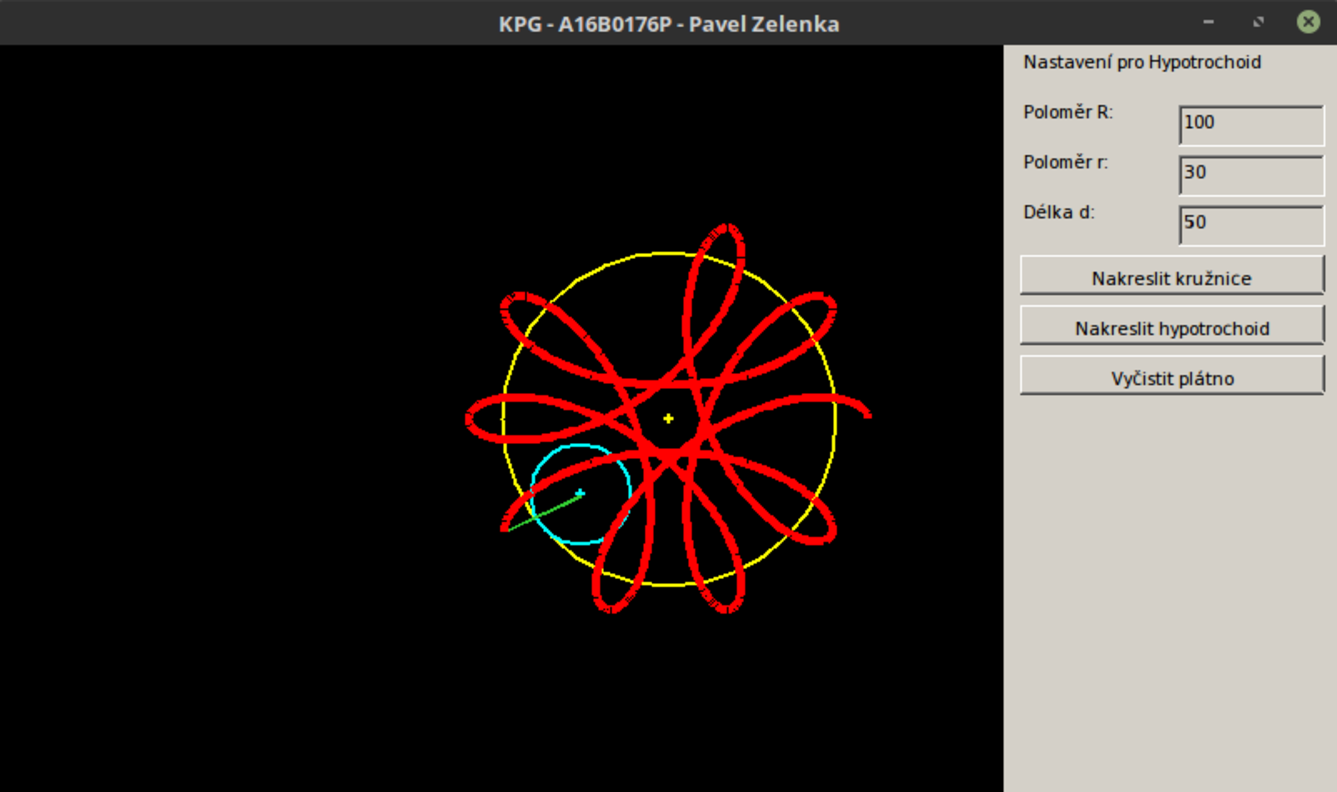
\includegraphics[width=0.9\textwidth,natwidth=1,natheight=1]{app_gui.pdf}
	\caption{Okno aplikace spuštěné pod Wine 3.2}
\end{figure}	

\newpage
\section{Závěr}
\paragraph{}
Úkol jsem řešil v\nobreakspace jazyce \texttt{C\#} s použitím \texttt{.NET Framework}.
V\nobreakspace oknu aplikace lze upřesňit parametry křivky. Všechny hodnoty jsou udávány v\nobreakspace pixelech. Aplikace provádí základní ošetření hodnot, zdali se\nobreakspace jedná o\nobreakspace čísla a zdali jsou v\nobreakspace intervalu datového typu.

\paragraph{}
Při změně rozměrů okna aplikace dojde k\nobreakspace zastavení animace. Ovládací prvky se při změně rozměrů okna nepřizpůsobí a zůstávají na svém místě. Tyto nedostatky plynnou z mé nezkušenosti s\nobreakspace \texttt{.NET Framework} a\nobreakspace s\nobreakspace aplikací  \texttt{Visual Studio}.

\paragraph{}
V\nobreakspace aplikaci je nastaven konstantní počet kroků pro průběh animace, křivka se však nemusí během tohoto času vrátit do výchozí polohy. Jako možné vylepšení aplikace se\nobreakspace proto nabízí zdokonalení výpočtu potřebných kroků animace.

\section{Reference}

Hypotrochoid – Wikipedie. [online]. Dostupné z: \href{https://en.wikipedia.org/wiki/Hypotrochoid}{en.wikipedia.org/wiki/Hypotrochoid}

\end{document}
